\documentclass{article}

\usepackage[serbian]{babel}
\usepackage[T1]{fontenc}
\usepackage[utf8]{inputenc}
\usepackage{geometry}
\usepackage[hidelinks]{hyperref}

\usepackage{amsmath,amssymb,amsthm}
\usepackage{graphicx}
\usepackage{float}  
\usepackage{xcolor}
\usepackage{listings}
\usepackage{algorithm}
\usepackage{algpseudocode}
\usepackage{tikz}
\usepackage{hyperref}
\usepackage{caption}
\usepackage{subcaption}
\usepackage{booktabs}
\usepackage{enumitem}
\usepackage{fancyhdr}

% ── Naslov ─────────────────────────────────────────────────
\title{\textbf{Površina unije pravougaonika}}
\author{Lana Matić 1009/2025\\
\small Matematički fakultet Univerziteta u Beogradu}
\date{}

\begin{document}
\maketitle

\section{Uvod}

Izračunavanje površine unije geometrijskih objekata jedan je od osnovnih problema u računarskoj geometriji. Problem se javlja u brojnim praktičnim primenama: u geografskim informacionim sistemima, u računarskoj grafici, u VLSI dizajnu integrisanih kola, kao i u robotici pri planiranju kretanja i analizi prostora.

U opštem slučaju, određivanje površine unije proizvoljnih poligona je složen problem. Međutim, kada su objekti pravougaonici čije su stranice paralelne koordinatnim osama (eng. \textit{axis-aligned rectangles}), problem dopušta efikasna rešenja zasnovana na tehnici brišuće prave (eng. \textit{sweep line}).

U ovom radu prikazan je algoritam brišuće prave sa kompresijom koordinata za rešavanje problema \textit{Rectangle Area II} (LeetCode 850). 


% ═══════════════════════════════════════════════════════════
\section{Opis problema}
% ═══════════════════════════════════════════════════════════

Dat je niz od $N$ pravougaonika u ravni čije su stranice paralelne koordinatnim osama. Svaki pravougaonik je definisan sa četiri celobrojna parametra:
\[
\texttt{rectangles}[i] = [x_1,\; y_1,\; x_2,\; y_2]
\]
gde je $(x_1, y_1)$ donji levi ugao, a $(x_2, y_2)$ gornji desni ugao.

\textbf{Zadatak:} Izračunati \textbf{ukupnu površinu} koju pokrivaju svi pravougaonici, pri čemu se svaka tačka ravni broji \textbf{samo jednom}, čak i ako je pokrivena sa više pravougaonika. Rezultat vratiti po modulu $10^9 + 7$.

\subsection{Primer}
Na slici~\ref{fig:example} su prikazana tri pravougaonika koja se delimično preklapaju. Naivnim sabiranjem površina dobijamo $4 + 2 + 2 = 8$, ali je tačan odgovor 6 jer se preklapajuće oblasti broje samo jednom.

\begin{figure}[H]
\centering
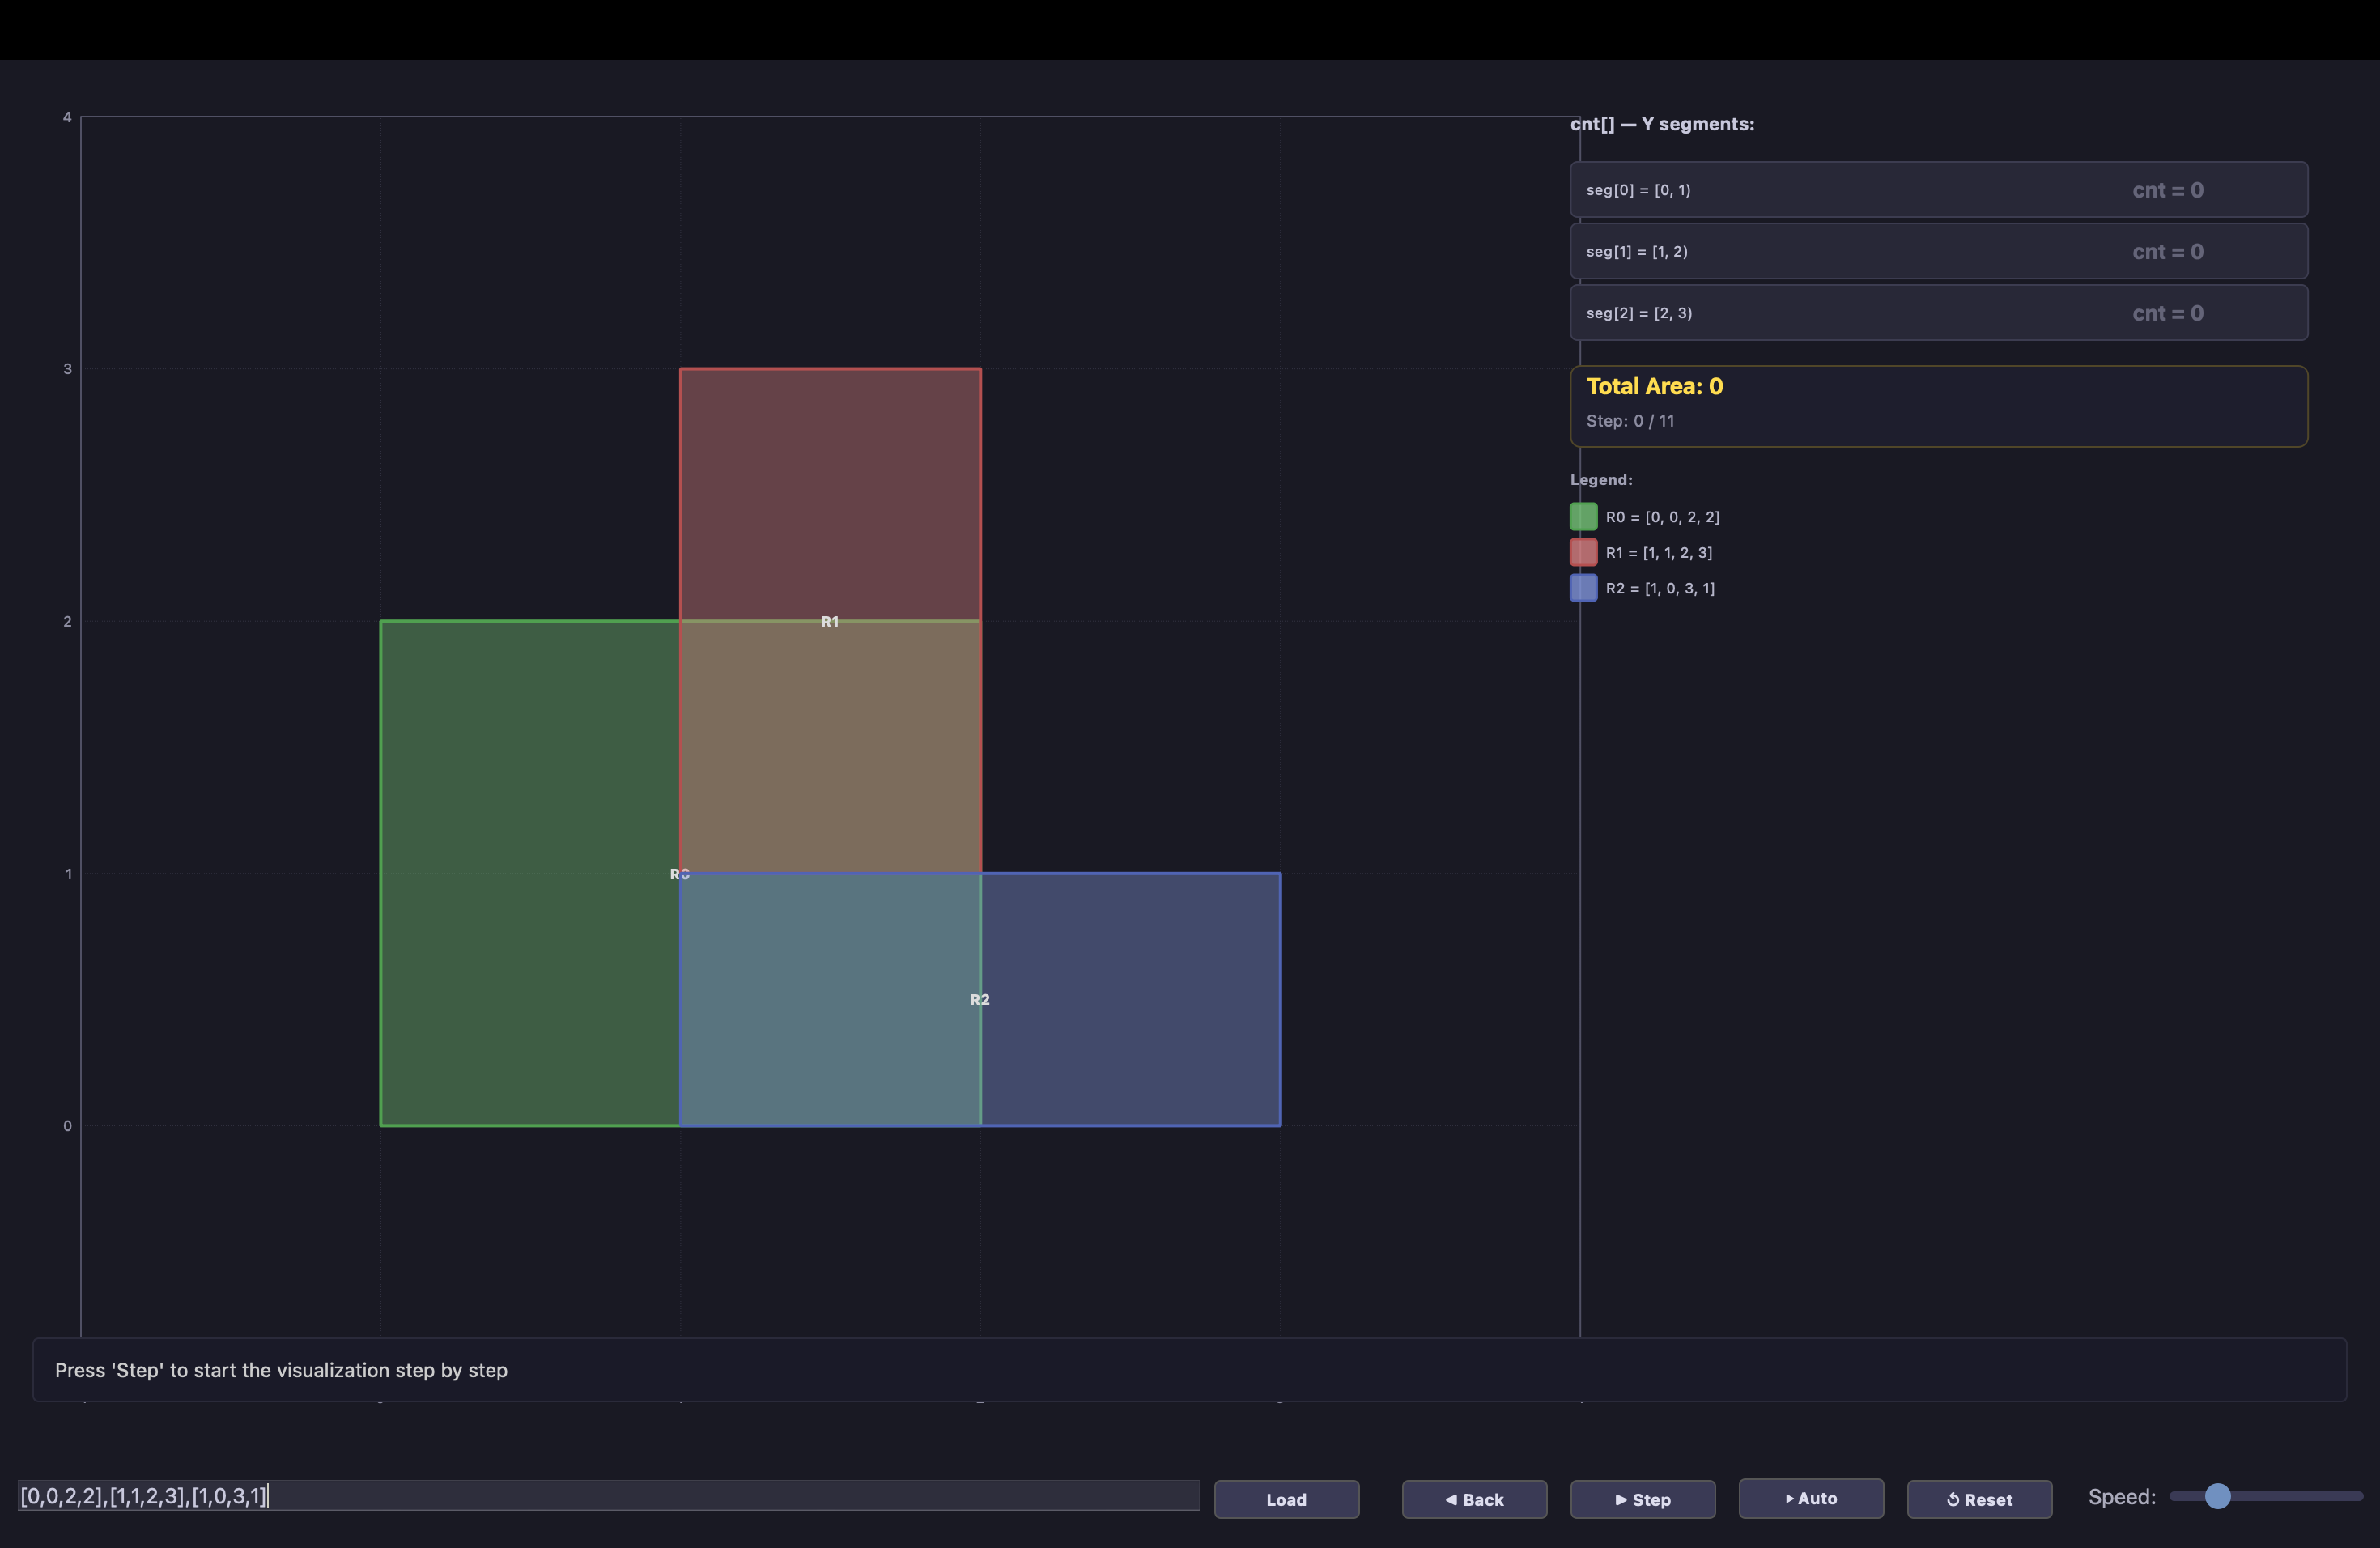
\includegraphics[width=0.75\textwidth]{../screenshots/example.png}
\caption{Ulaz: \texttt{[[0,0,2,2], [1,1,2,3], [1,0,3,1]]}. Površina po modulu $10^9 + 7$ je \textbf{6}.}
\label{fig:example}
\end{figure}


% ═══════════════════════════════════════════════════════════
\section{Algoritam: Brišuća prava sa kompresijom koordinata}
% ═══════════════════════════════════════════════════════════
Za rešenje problema korišćen je algoritam brišuće prave koja se kreće s leva na desno duž $x$-ose uz kompresiju koordinata. U svakom trenutku, brišuća prava preseca određene pravougaonike. Delovi linije koji su unutar bar jednog pravougaonika čine \textit{aktivnu visinu}.

Površina se računa kao suma proizvoda širine svake vertikalne trake i njene aktivne visine:
\[
\text{Ukupna površina} = \sum_{\text{trake}} \underbrace{(x_{i+1} - x_i)}_{\text{širina}} \cdot \underbrace{h_{\text{aktivna}}}_{\text{visina}}
\]

\subsection{Korak 1: Kompresija Y koordinata}

Iz svih pravougaonika izvlačimo jedinstvene $Y$ koordinate i sortiramo ih. One definišu \textit{$Y$-segmente} - intervale čija se pokrivenost prati tokom prelaza.

Za primer sa slike~\ref{fig:example}:
\[
Y = \{0, 1, 2, 3\} \quad \Rightarrow \quad \text{segmenti:}\; [0,1),\; [1,2),\; [2,3)
\]

Niz $\texttt{cnt}[i]$ broji koliko pravougaonika trenutno pokriva segment $i$. Segment je \textit{aktivan} ako je $\texttt{cnt}[i] > 0$.

\subsection{Korak 2: Kreiranje događaja}

Za svaki pravougaonik $[x_1, y_1, x_2, y_2]$ kreiramo dva \textit{događaja} (events):
\begin{itemize}[nosep]
    \item \textbf{START} na $x = x_1$ - pravougaonik počinje da pokriva interval $[y_1, y_2)$
    \item \textbf{END} na $x = x_2$ - pravougaonik prestaje da pokriva interval $[y_1, y_2)$
\end{itemize}

Događaji se sortiraju po $x$-koordinati.

\subsection{Korak 3: Obrada događaja}

Prolazimo kroz događaje s leva na desno. Za svaku traku između dva uzastopna događaja:

\begin{enumerate}[nosep]
    \item Izračunamo \textit{aktivnu visinu} - sumu realnih visina svih segmenata sa $\texttt{cnt}[i] > 0$
    \item Pomnožimo širinu trake sa aktivnom visinom i dodamo u ukupnu površinu
    \item Ažuriramo niz $\texttt{cnt}[]$ na osnovu tekućeg događaja
\end{enumerate}

% ═══════════════════════════════════════════════════════════
\section{Analiza složenosti}
% ═══════════════════════════════════════════════════════════

Neka je $N$ broj pravougaonika (ograničenje: $N \leq 200$).

\subsection{Vremenska složenost: $O(N^2)$}

\begin{table}[H]
\centering
\begin{tabular}{lll}
\toprule
Faza & Operacija & Složenost \\
\midrule
Kompresija $Y$ koordinata & Sortiranje $2N$ vrednosti & $O(N \log N)$ \\
Kreiranje događaja & $2N$ događaja & $O(N)$ \\
Sortiranje događaja & Sortiranje po $x$ & $O(N \log N)$ \\
\textbf{Brišuća prava} & \textbf{$2N$ događaja $\times$ $O(N)$ po događaju} & $\boldsymbol{O(N^2)}$ \\
\bottomrule
\end{tabular}
\caption{Vremenska složenost po fazama algoritma.}
\label{tab:complexity}
\end{table}

Kao što je prikazano u tabeli~\ref{tab:complexity}, dominantan član je faza brišuće prave. Za svaki od $2N$ događaja:
\begin{itemize}[nosep]
    \item Računanje aktivne visine zahteva prolazak kroz ceo $\texttt{cnt}[]$ niz dužine $O(N)$
    \item Ažuriranje $\texttt{cnt}[]$ za jedan pravougaonik zahteva prolazak kroz do $O(N)$ segmenata
\end{itemize}

Dakle: $O(N)$ događaja $\times$ $O(N)$ po događaju $= O(N^2)$.

Za $N = 200$, to je $\sim 80\,000$ operacija - gotovo trenutno.

\subsection{Prostorna složenost: $O(N)$}

\begin{itemize}[nosep]
    \item $\texttt{yVals}[]$: $O(N)$ jedinstvenih koordinata
    \item $\texttt{cnt}[]$: $O(N)$ segmenata
    \item $\texttt{events}[]$: $O(N)$ događaja
    \item $\texttt{states}[]$: $O(N)$ stanja (za vizualizaciju)
\end{itemize}

\subsection{Modularna aritmetika}

Koordinate mogu biti do $10^9$, pa je maksimalna površina jednog pravougaonika do $10^{18}$, što staje u \texttt{long long} ($\sim 9.2 \times 10^{18}$). Međutim, zadatak traži rezultat modulo $10^9 + 7$:
\[
\texttt{ans} = \left(\texttt{ans} + (\texttt{width} \bmod M) \cdot (\texttt{activeH} \bmod M)\right) \bmod M, \quad M = 10^9 + 7
\]

Primer primene modularne aritmetike prikazan je na slici~\ref{fig:big}, gde pravougaonik sa koordinatama do $10^9$ daje površinu $10^{18}$, a rezultat po modulu je 49.

\subsection{Struktura projekta}

Algoritam je odvojen od vizualizacije - \texttt{algorithm\_solution.h/cpp} nema nikakvu zavisnost od Qt biblioteke i može se koristiti samostalno ili kao biblioteka za bilo koji frontend.

\begin{table}[H]
\centering
\begin{tabular}{ll}
\toprule
Fajl & Opis \\
\midrule
\texttt{algorithm\_solution.h/cpp} & Čist C++ --- algoritam brišuće prave \\
\texttt{mainwindow.h/cpp/ui} & Qt vizualizacija --- crtanje i kontrole \\
\texttt{main.cpp} & Entry point sa tamnom temom \\
\texttt{CMakeLists.txt} & Build konfiguracija \\
\bottomrule
\end{tabular}
\caption{Struktura projekta.}
\label{tab:structure}
\end{table}

% ═══════════════════════════════════════════════════════════
\section{Qt vizualizacija}
% ═══════════════════════════════════════════════════════════

Vizualizacija omogućava korak-po-korak praćenje rada algoritma. Korisnik unosi pravougaonike u tekstualno polje i koristi kontrole za navigaciju kroz stanja algoritma.
Na slici~\ref{fig:viz} prikazana su dva karakteristična stanja vizualizacije: početno stanje pre pokretanja algoritma (slika~\ref{fig:viz-init}) i stanje u koraku 9 od 11, kada je brišuća prava stigla do $x = 3$ (slika~\ref{fig:viz-sweep}).

\begin{figure}[H]
\centering
\begin{subfigure}[t]{0.48\textwidth}
    \centering
    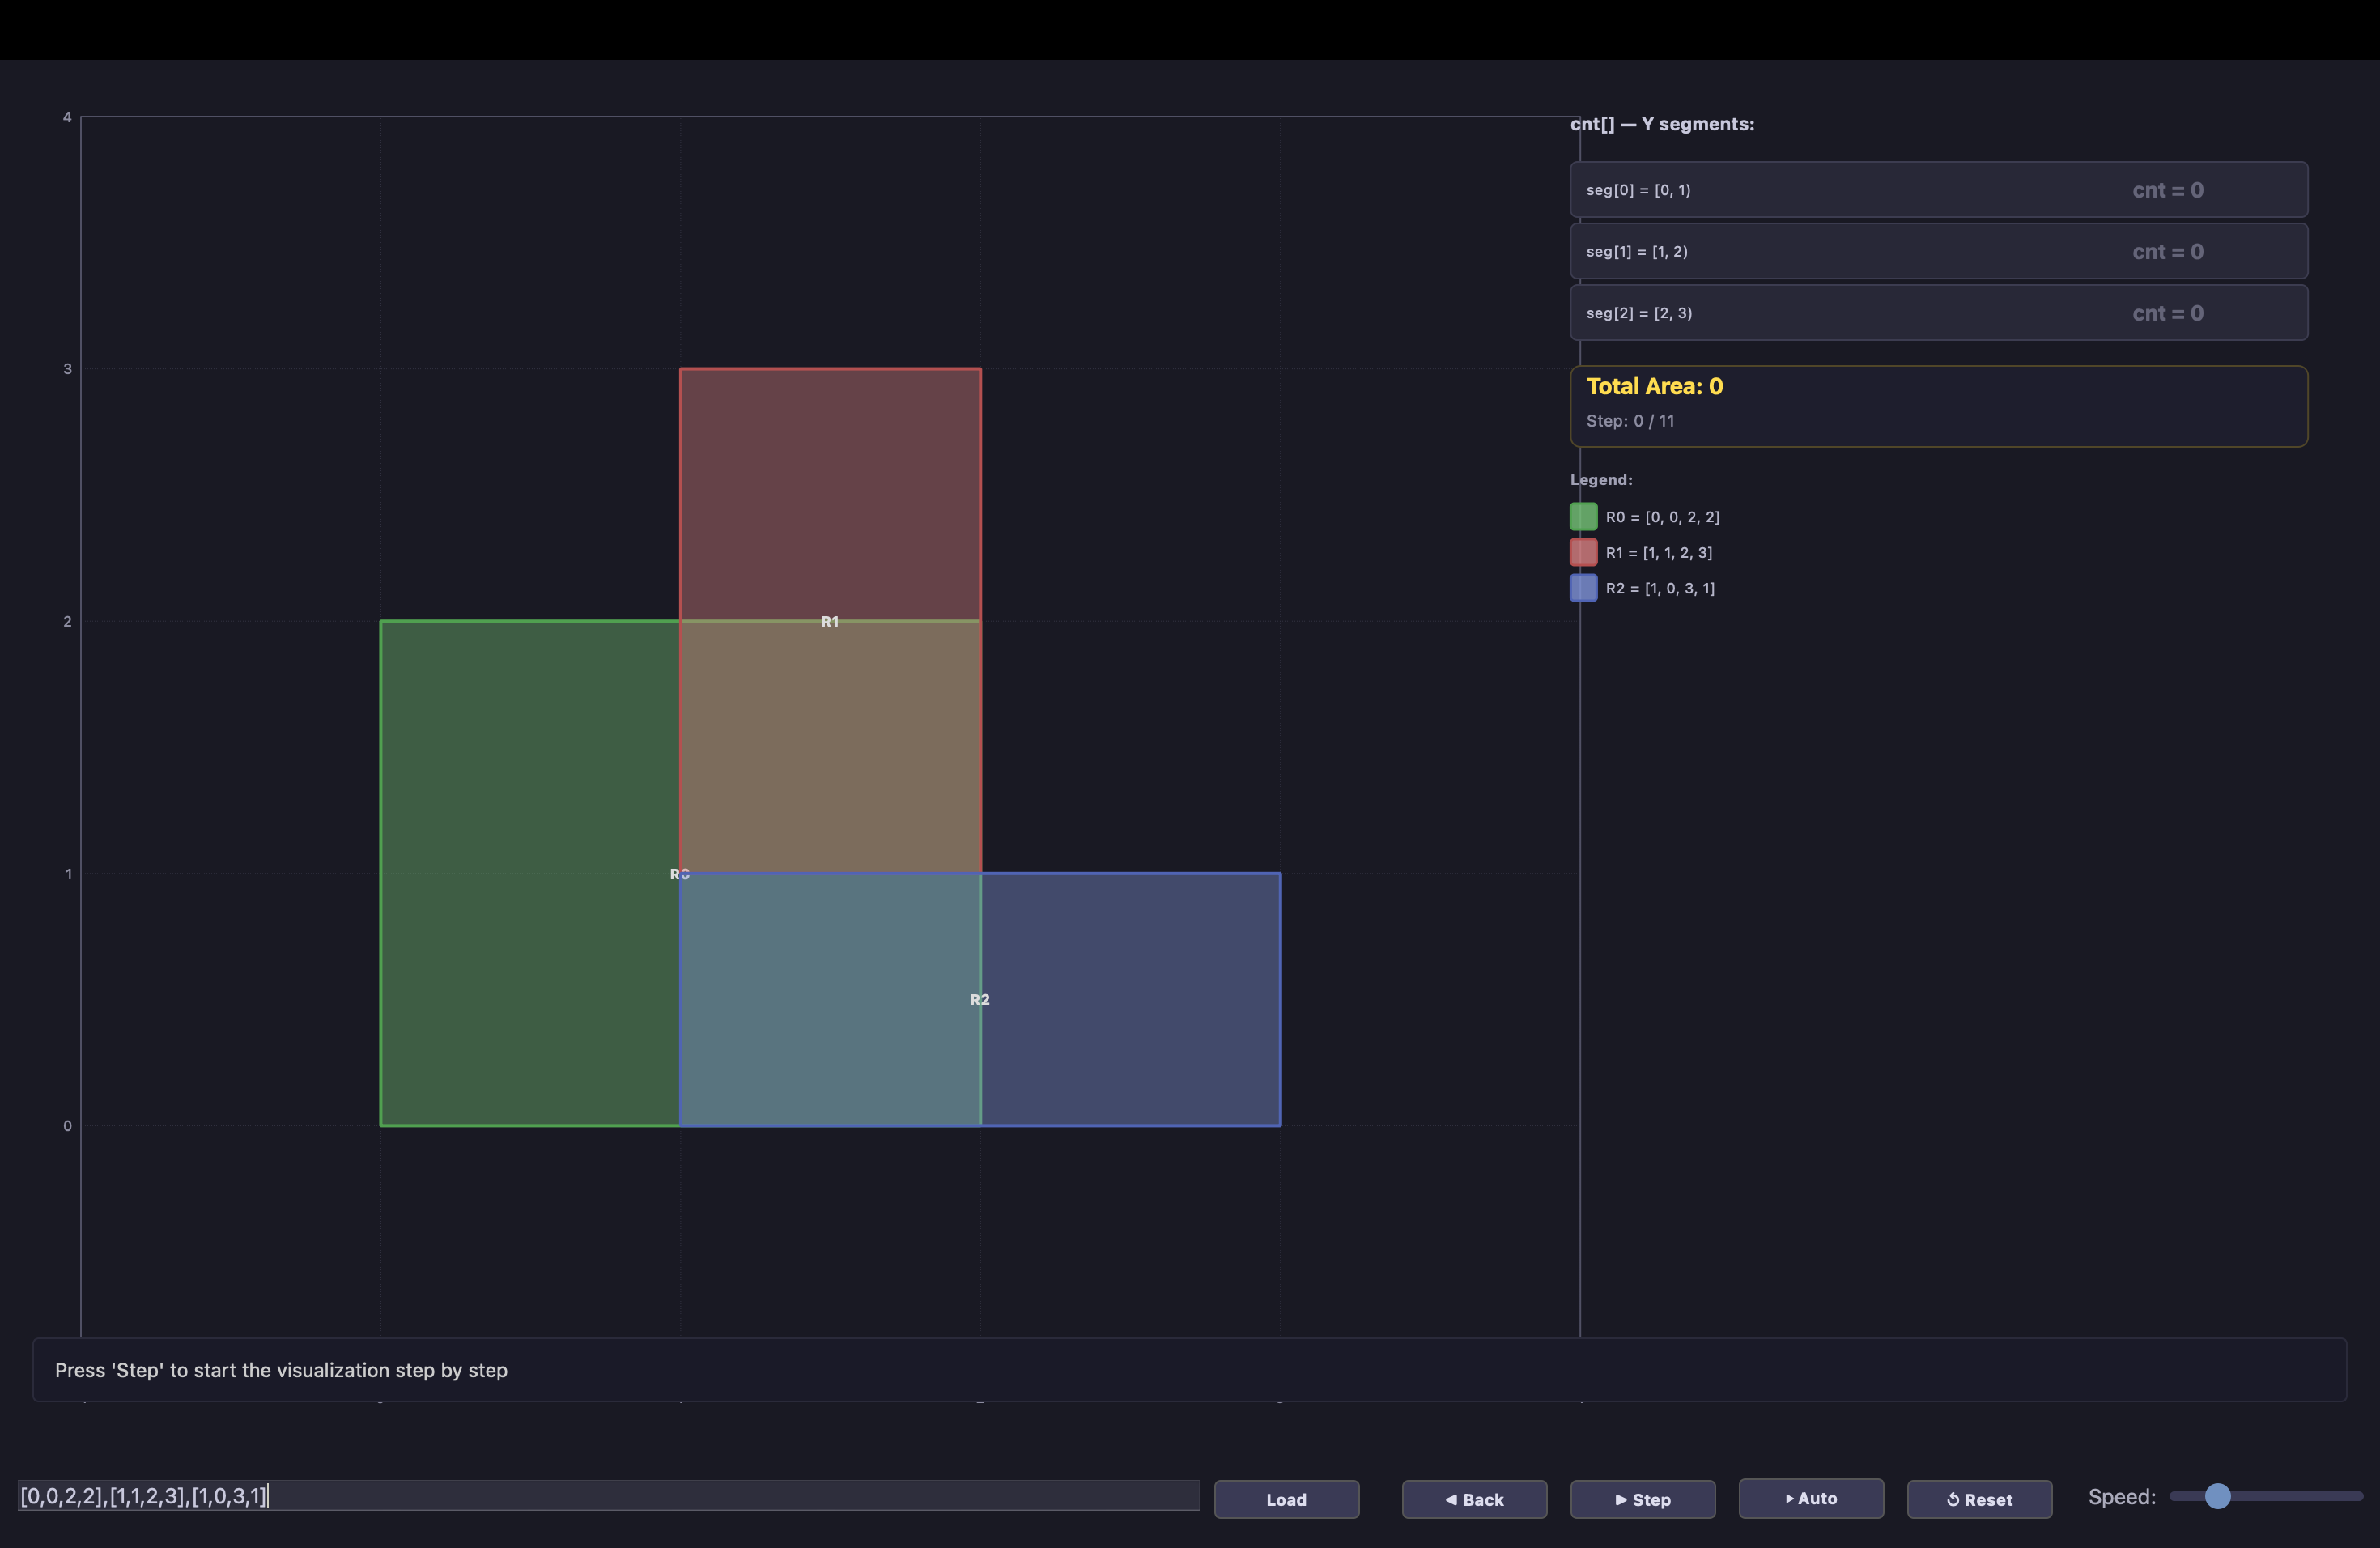
\includegraphics[width=\textwidth]{../screenshots/example.png}
    \caption{Početno stanje - pravougaonici učitani, \texttt{cnt[]} svi nule, vizualizacija spremna.}
    \label{fig:viz-init}
\end{subfigure}
\hfill
\begin{subfigure}[t]{0.48\textwidth}
    \centering
    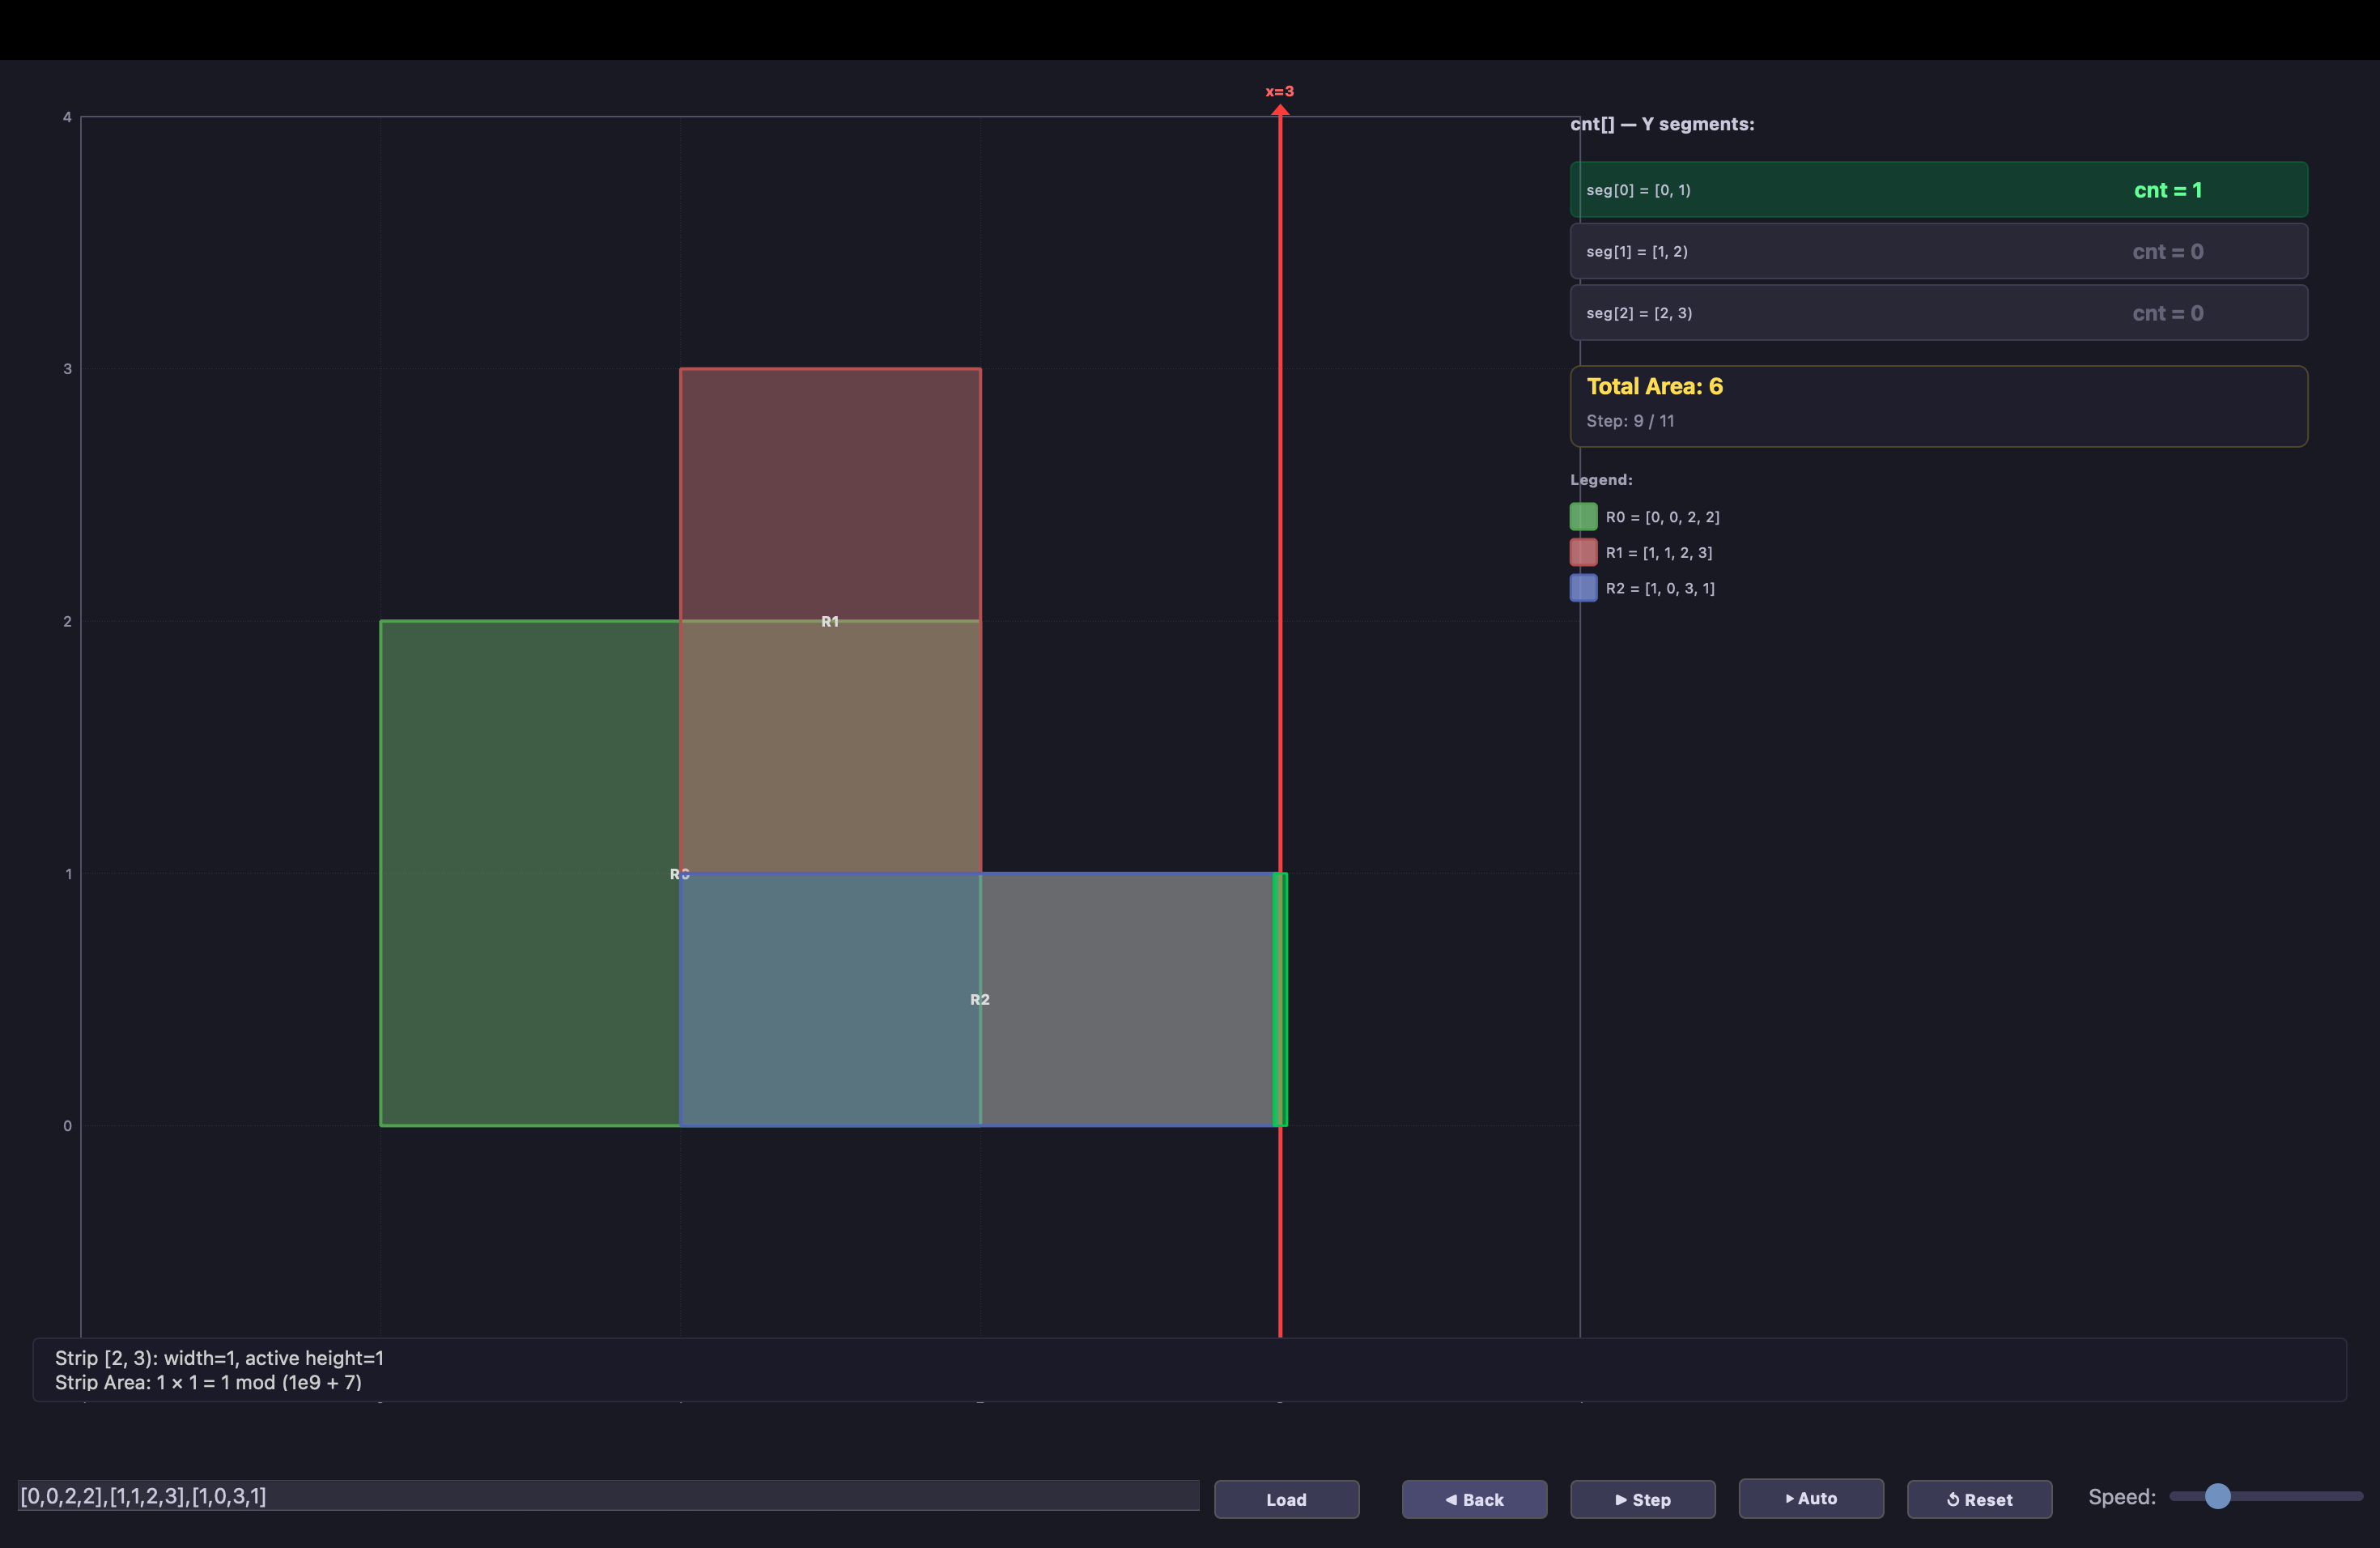
\includegraphics[width=\textwidth]{../screenshots/sweepline.png}
    \caption{Brišuća prava na $x{=}3$ (korak 9/11). Zeleni segment pokazuje aktivan $[0,1)$. Ukupna površina: 6.}
    \label{fig:viz-sweep}
\end{subfigure}
\caption{Vizualizacija za primer \texttt{[0,0,2,2],[1,1,2,3],[1,0,3,1]}}
\label{fig:viz}
\end{figure}

\subsection{Elementi vizualizacije}

\begin{itemize}[nosep]
    \item \textbf{Levi panel} --- koordinatna mreža sa obojenim pravougaonicima (providne boje za prikaz preklapanja)
    \item \textbf{Crvena sweep linija} --- trenutna $x$-pozicija, kreće se s leva na desno
    \item \textbf{Žute trake} --- oblast čija se površina upravo računa
    \item \textbf{Zeleni segmenti na sweep liniji} --- aktivni $Y$-segmenti ($\texttt{cnt}[i] > 0$)
    \item \textbf{Desni panel} --- $\texttt{cnt}[]$ niz, zeleno osvetljen kad je segment aktivan
    \item \textbf{Ukupna površina} --- tekući zbir sa rezultatom modulo $10^9 + 7$
\end{itemize}

\subsection{Rad sa velikim koordinatama}

\begin{figure}[H]
\centering
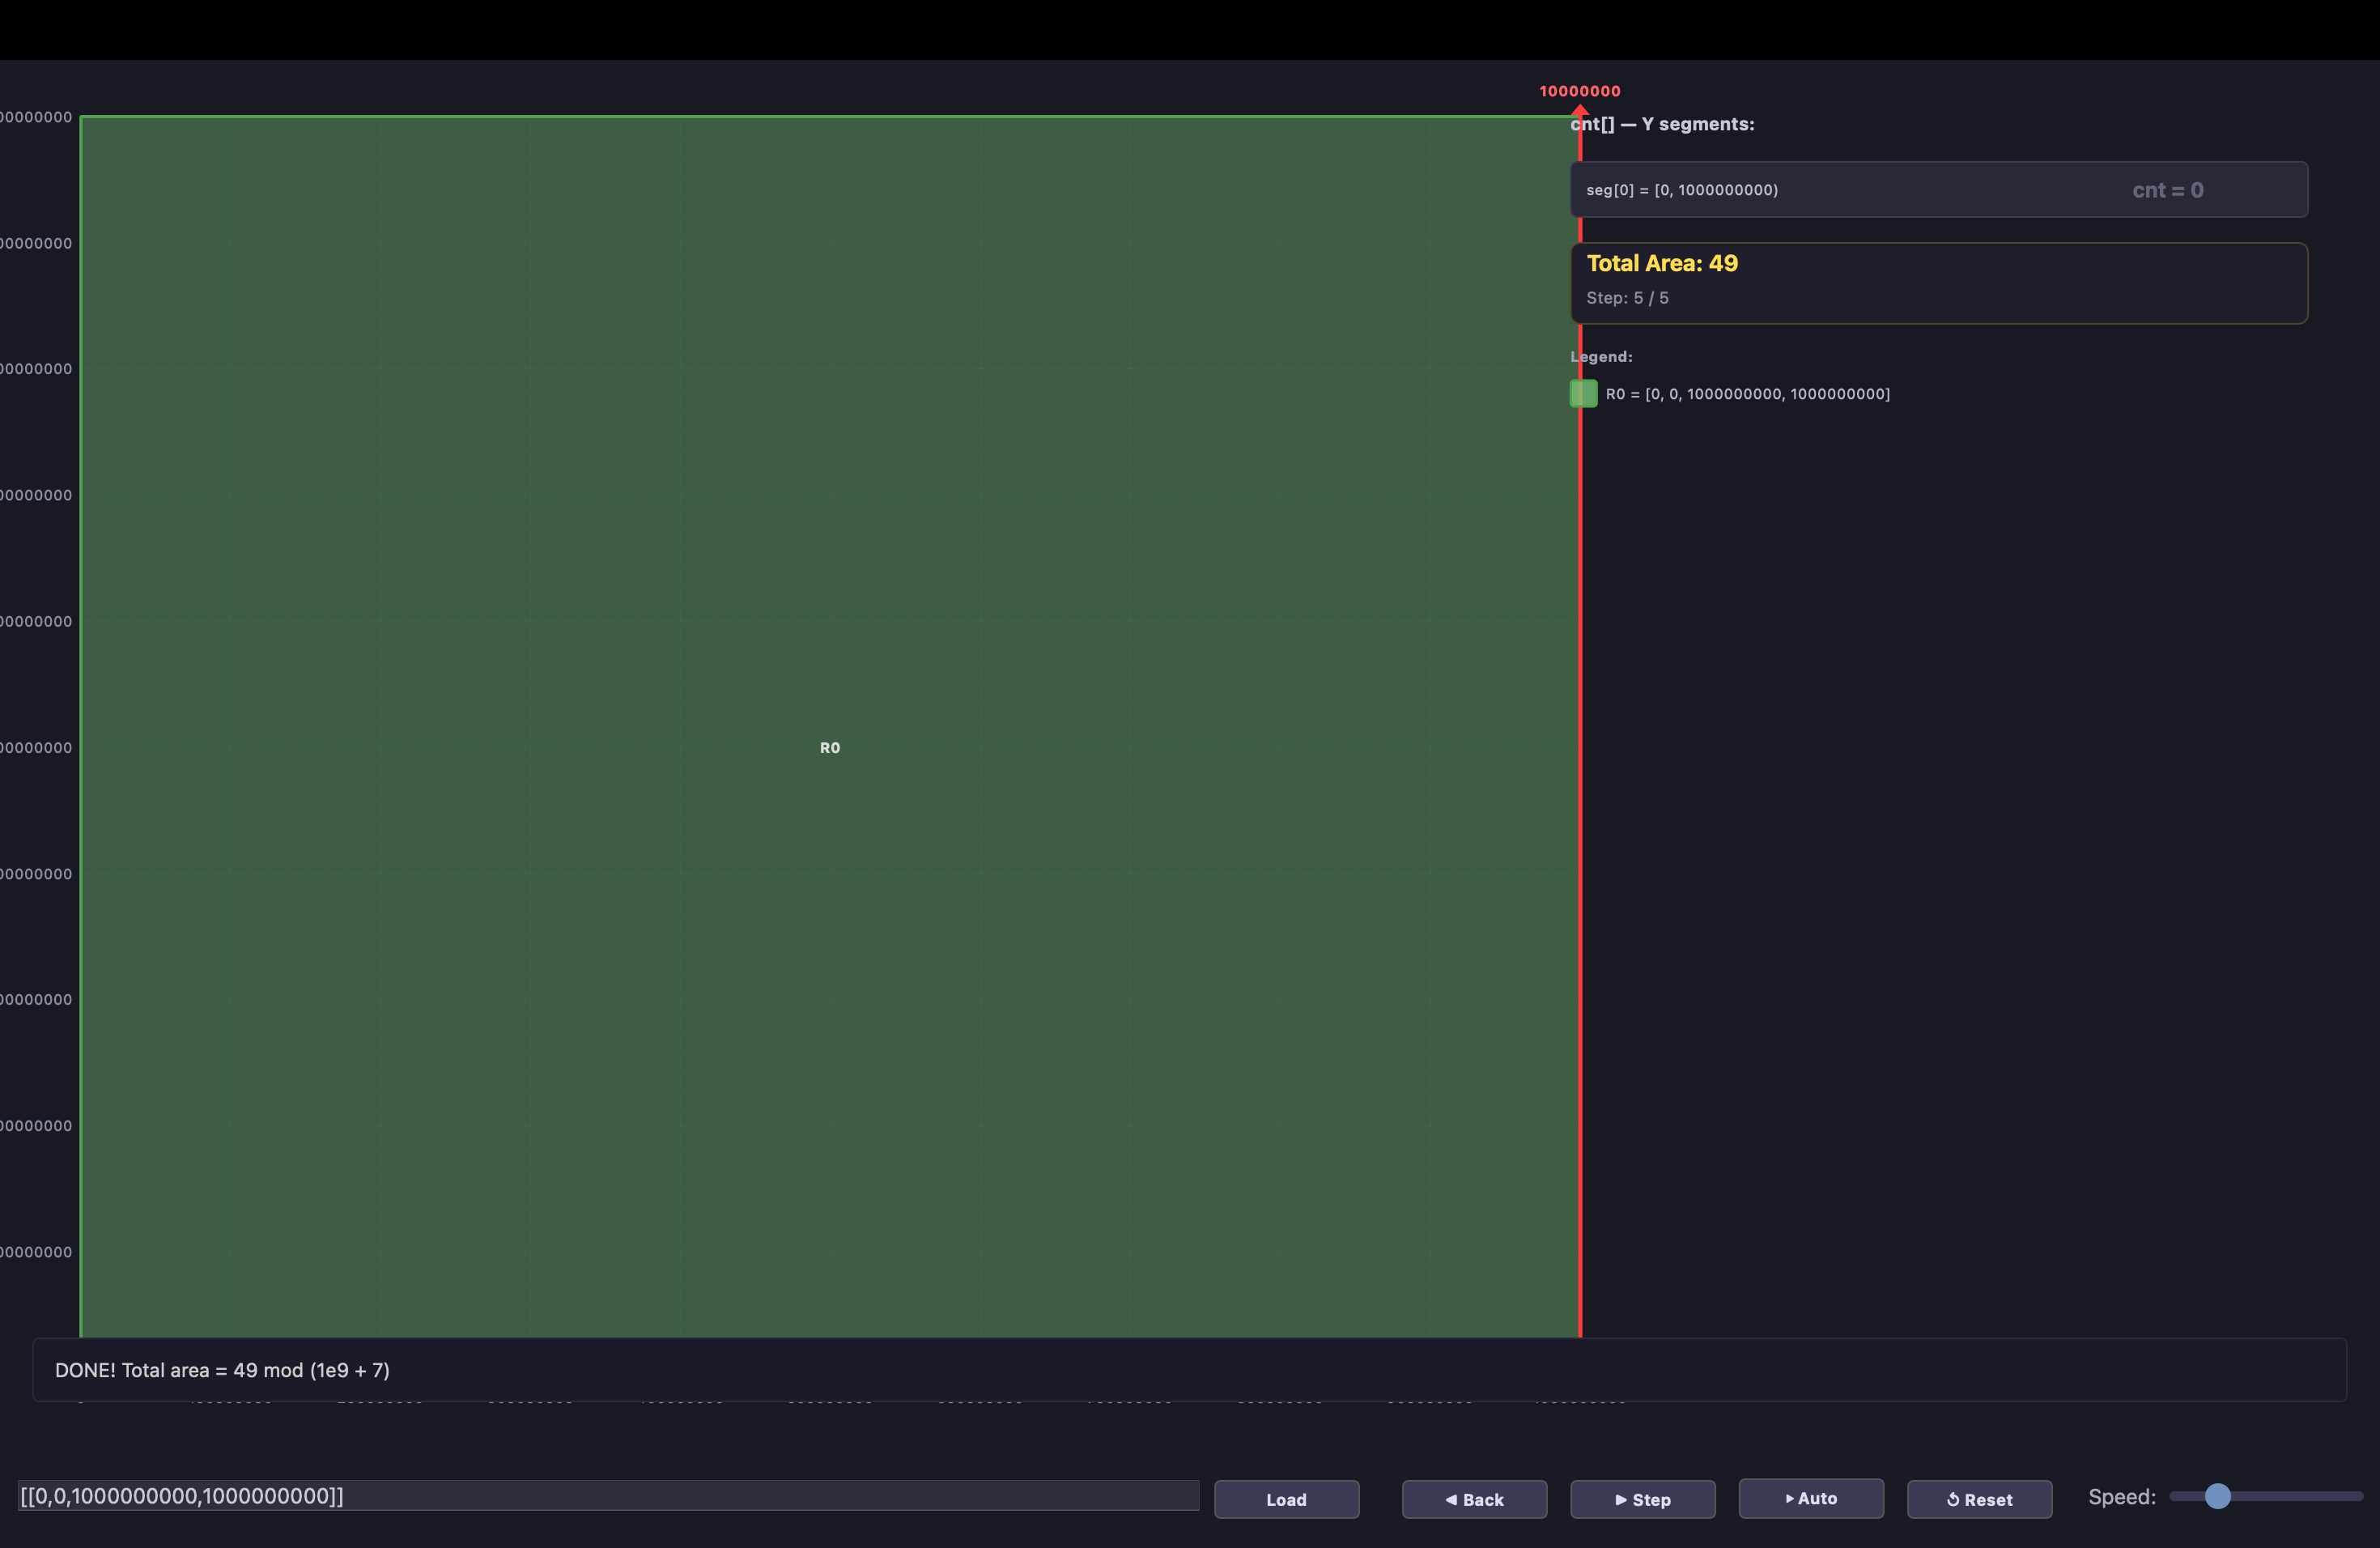
\includegraphics[width=0.75\textwidth]{../screenshots/big.png}
\caption{Ulaz: \texttt{[0,0,1000000000,1000000000]}. Površina iznosi $10^{18}$, a rezultat po modulu $10^9 + 7$ je \textbf{49}. Adaptivna mreža automatski bira odgovarajuće korake za ose.}
\label{fig:big}
\end{figure}

% ═══════════════════════════════════════════════════════════
\section{Zaključak}
% ═══════════════════════════════════════════════════════════

U ovom radu prikazan je algoritam brišuće prave za izračunavanje površine unije pravougaonika čije su stranice paralelne koordinatnim osama. Algoritam koristi kompresiju koordinata kako bi sveo beskonačan koordinatni prostor na konačan skup segmenata, a zatim brišuću pravu za efikasno praćenje pokrivenih oblasti.

Implementacija u jeziku C++ je razdvojena na algoritamski deo (bez zavisnosti od eksternih biblioteka) i vizualizacioni deo (Qt framework), što omogućava nezavisno testiranje i lako proširivanje.

Za ograničenje $N \leq 200$, složenost $O(N^2)$ je potpuno zadovoljavajuća.

\end{document}
